\documentclass[8pt,a4paper,compress]{beamer}

\usepackage{/home/siyer/lib/slides}

\title{Undirected Graphs}
\date{}
\begin{document}
\begin{frame}
\vfill
\titlepage
\end{frame}

\begin{frame}
\frametitle{Outline}
\tableofcontents
\end{frame}

\section{What are Graphs?}
\begin{frame}[fragile]
A \emph{graph} is a set of $V$ vertices connected pairwise by $E$ edges

\smallskip

\begin{center}
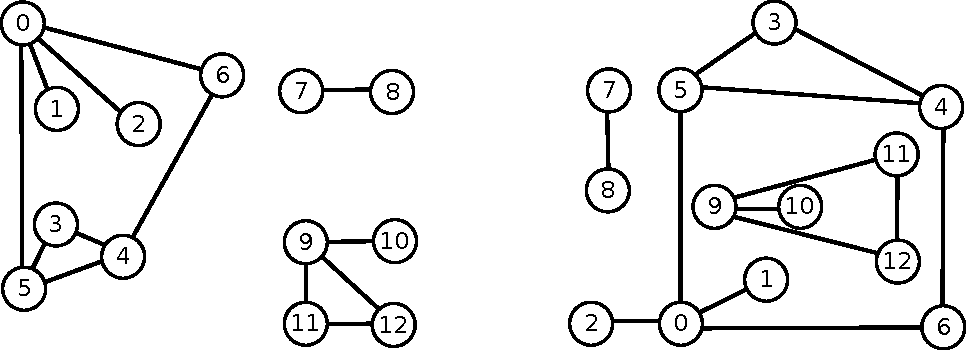
\includegraphics[scale=0.4]{{./figures/graph1}.png}
\end{center}

\bigskip

We use the names 0 through $V-1$ for the vertices in a $V$-vertex graph

\bigskip

We use the notation $v$-$w$ to refer to an edge that connects vertices $v$ and $w$

\bigskip

A \emph{self-loop} is an edge that connects a vertex to itself

\bigskip

\emph{Parallel edges} are edges that connect the same pair of vertices  
\end{frame}

\begin{frame}[fragile]
\begin{minipage}{220pt}
The \emph{degree} of a vertex is the number of vertices connected to it

\bigskip

A \emph{path} is a sequence of vertices connected by edges

\bigskip

A \emph{cycle} is a path with at least one edge whose first and last vertices are the same

\bigskip

The \emph{length} of a path or a cycle is its number of edges

\bigskip

A graph is \emph{connected} if there is a path from every vertex to every other vertex in the graph

\bigskip

A graph that is not connected consists of a set of \emph{connected components}, which are maximal connected subgraphs

\bigskip

An \emph{acyclic graph} is a graph with no cycles

\bigskip

A \emph{tree} is an acyclic connected graph

\bigskip

A \emph{bipartite graph} is a graph whose vertices can be divided into two sets such that all edges connect a vertex in one set with a vertex in the other set
\end{minipage}%
\begin{minipage}{100pt}
\begin{center}
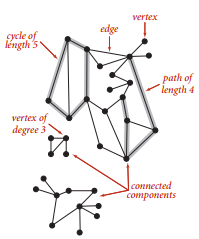
\includegraphics[scale=0.45]{{./figures/graph2}.png}

\tiny anatomy of a graph

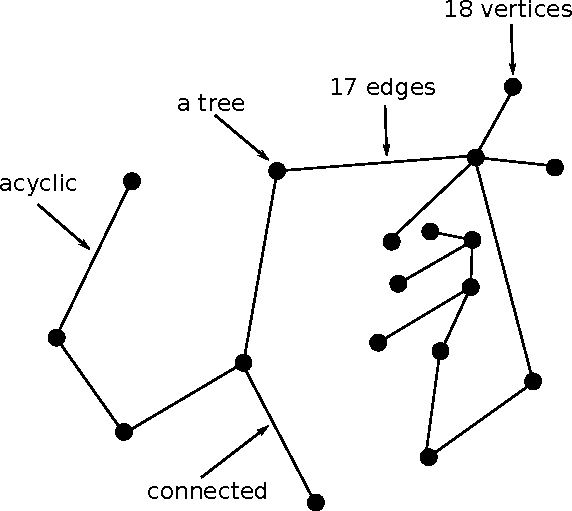
\includegraphics[scale=0.45]{{./figures/graph3}.png}

\tiny a tree

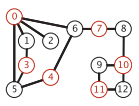
\includegraphics[scale=0.45]{{./figures/bipartite}.png}

\tiny a bipartite graph
\end{center}
\end{minipage}
\end{frame}

\begin{frame}[fragile]
Graph applications
\begin{center}
\begin{tabular}{ccc}
graph & vertex & edge \\ \hline \\
communication & telephone, computer & fiber optic cable \\
circuit & gate, register, processor & wire \\
mechanical & joint & rod, beam, spring \\
financial & stock, currency & transactions \\
transportation & intersection & street \\
internet & class C network & connection \\
game & board position & legal move \\
social relationship & person & friendship \\
neural network & neuron & synapse \\
protein network & protein & protein-protein interaction \\
molecule & atom & bond
\end{tabular}  
\end{center}
\end{frame}

\begin{frame}[fragile]
Example: Internet graph

\smallskip

\begin{center}
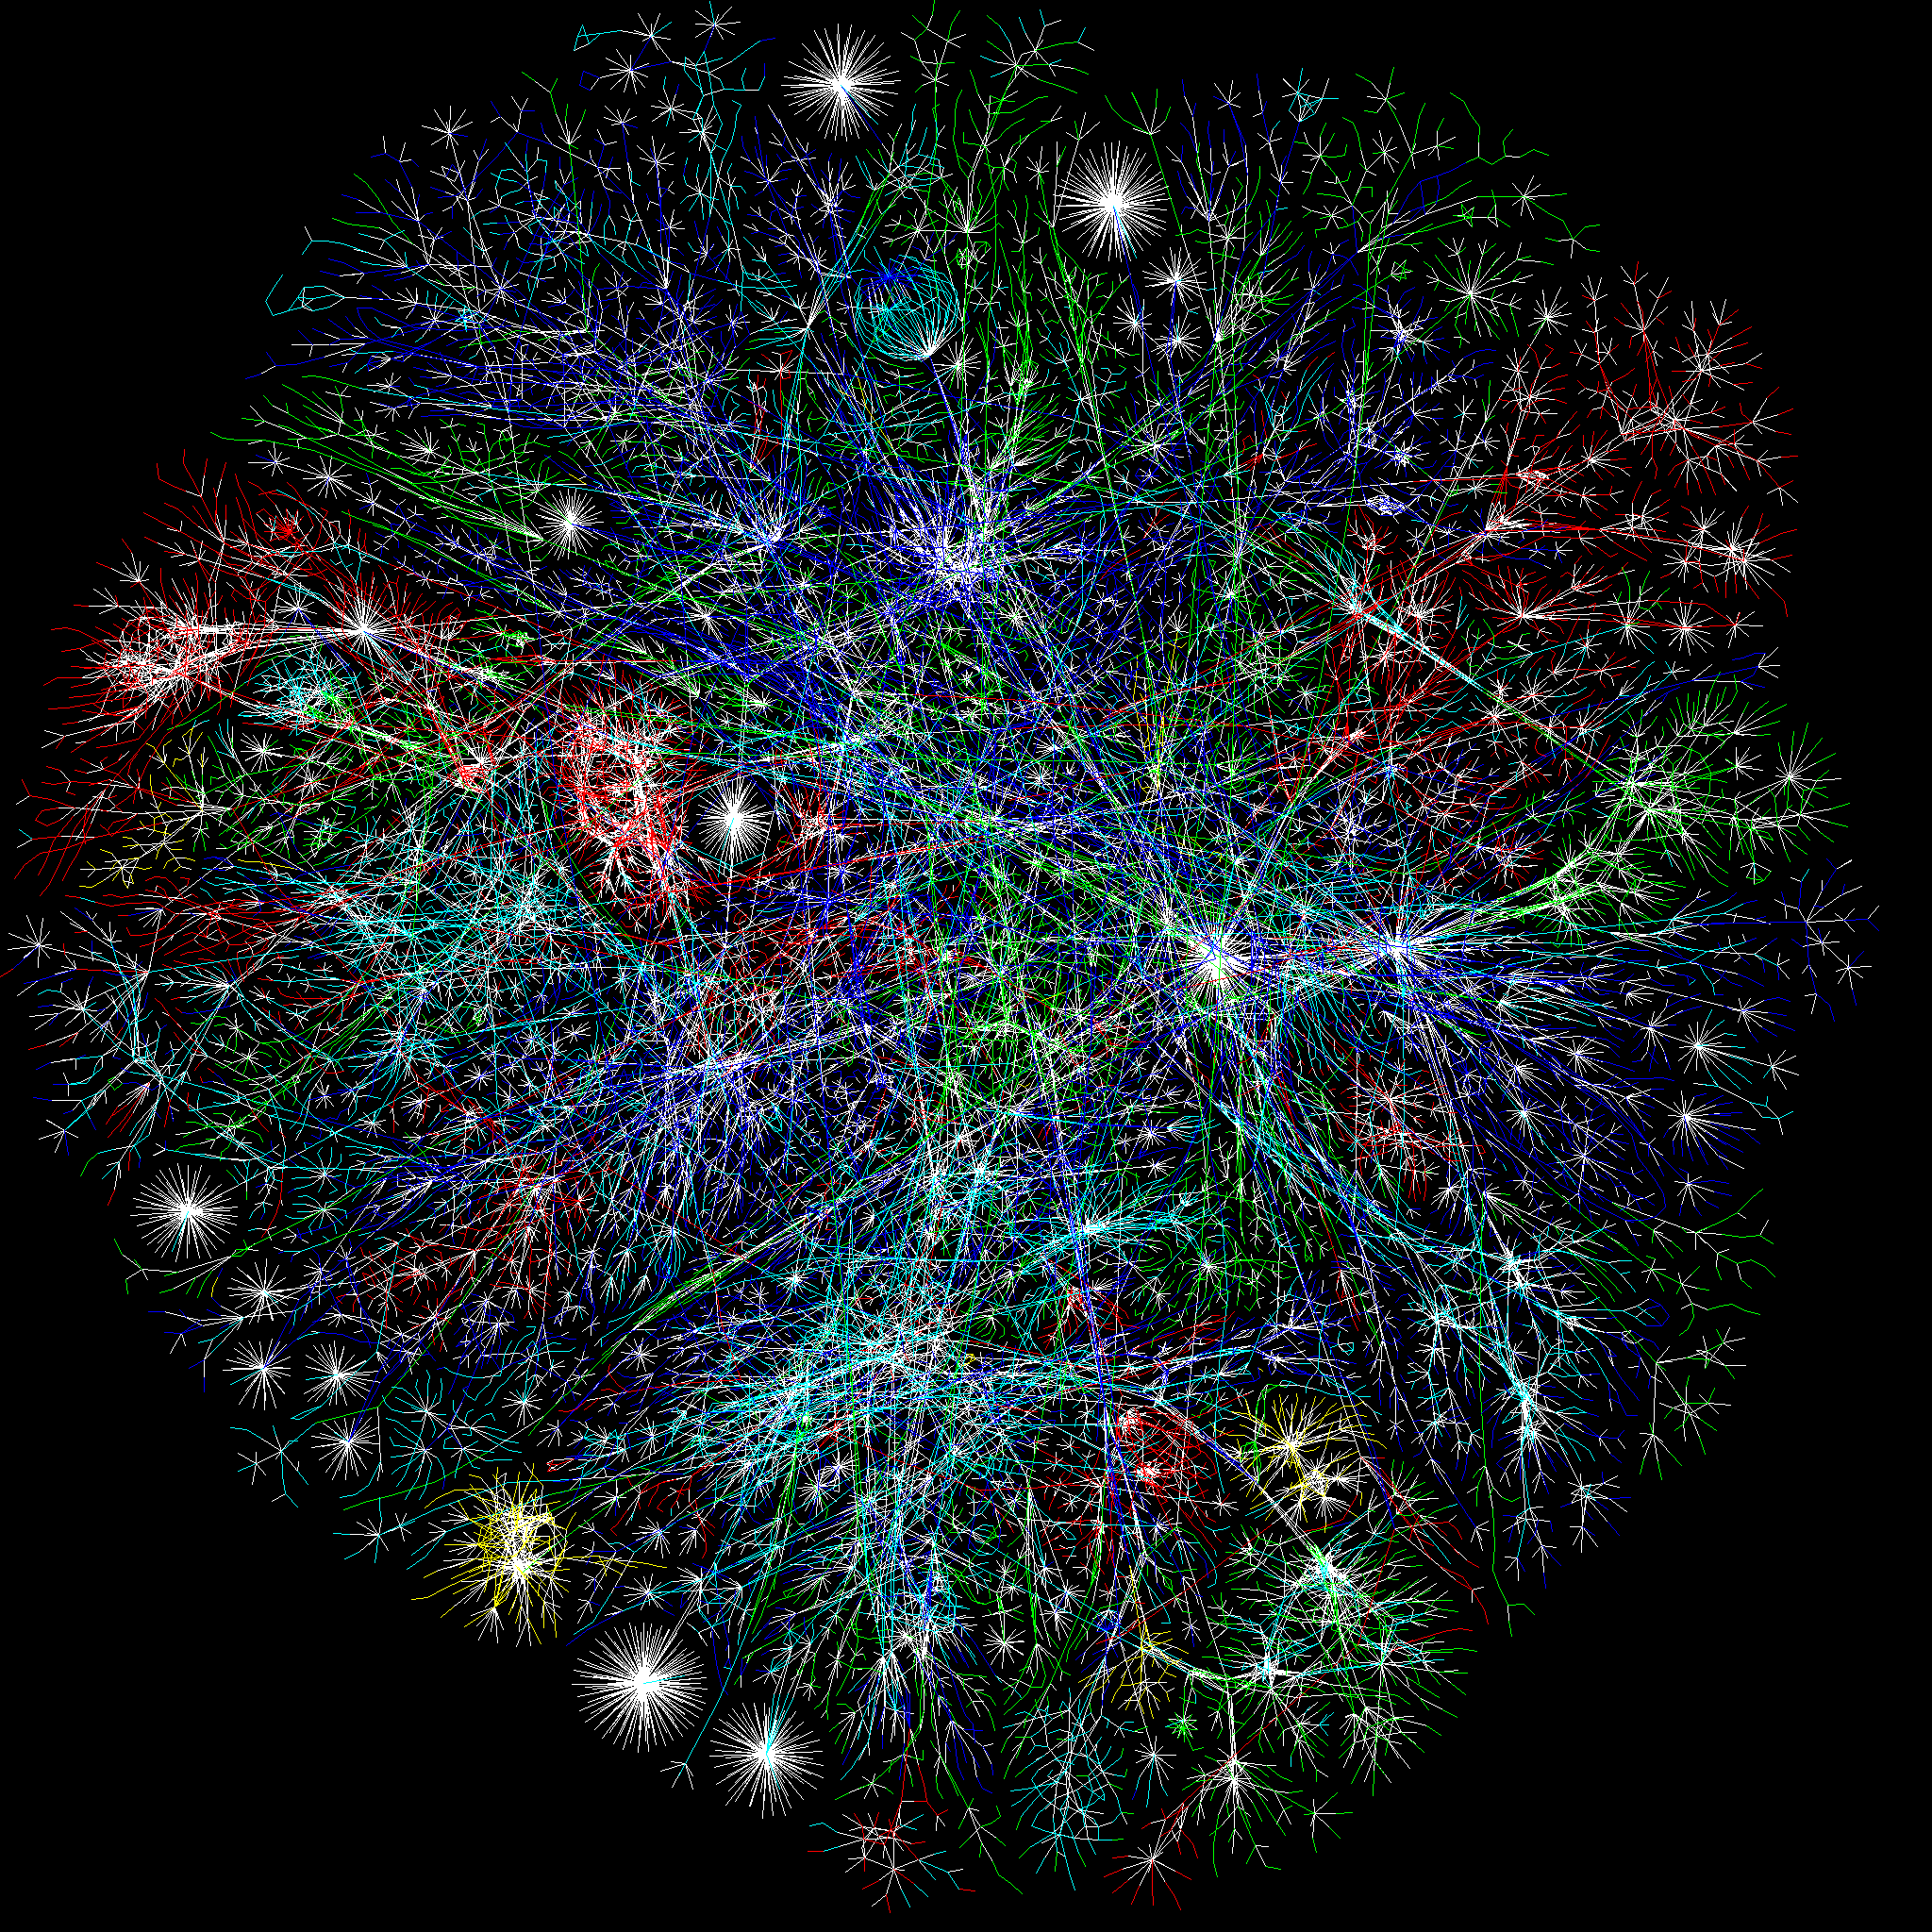
\includegraphics[scale=0.1]{{./figures/internet}.png}
\end{center}
\end{frame}

\begin{frame}[fragile]
Example: facebook graph

\smallskip

\begin{center}
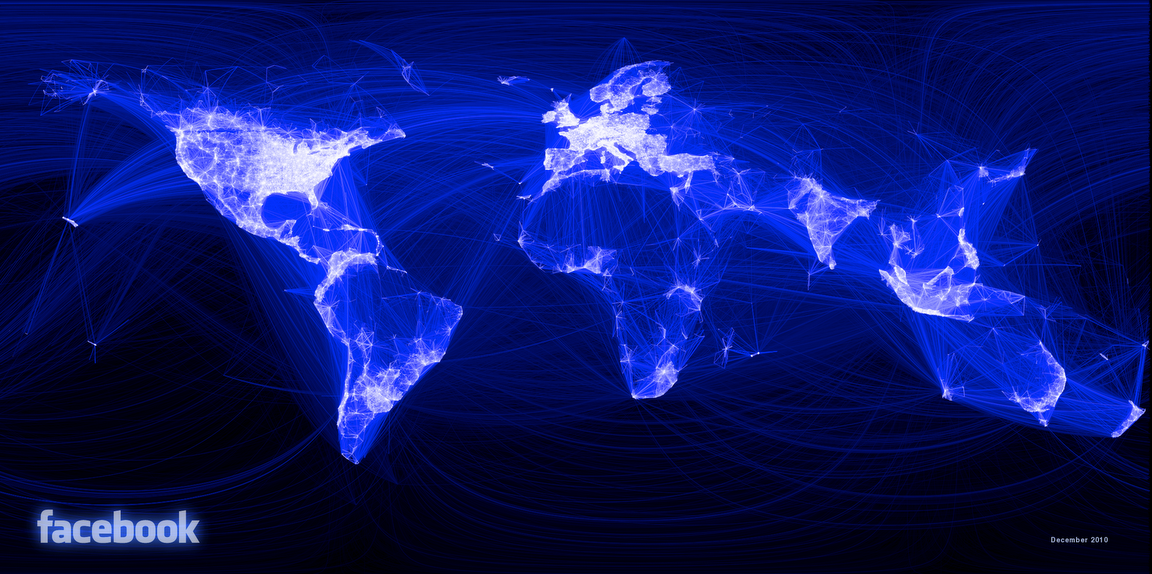
\includegraphics[scale=0.25]{{./figures/facebook}.png}
\end{center}
\end{frame}

\begin{frame}[fragile]
Example: c.elegans connectome graph

\smallskip

\begin{center}
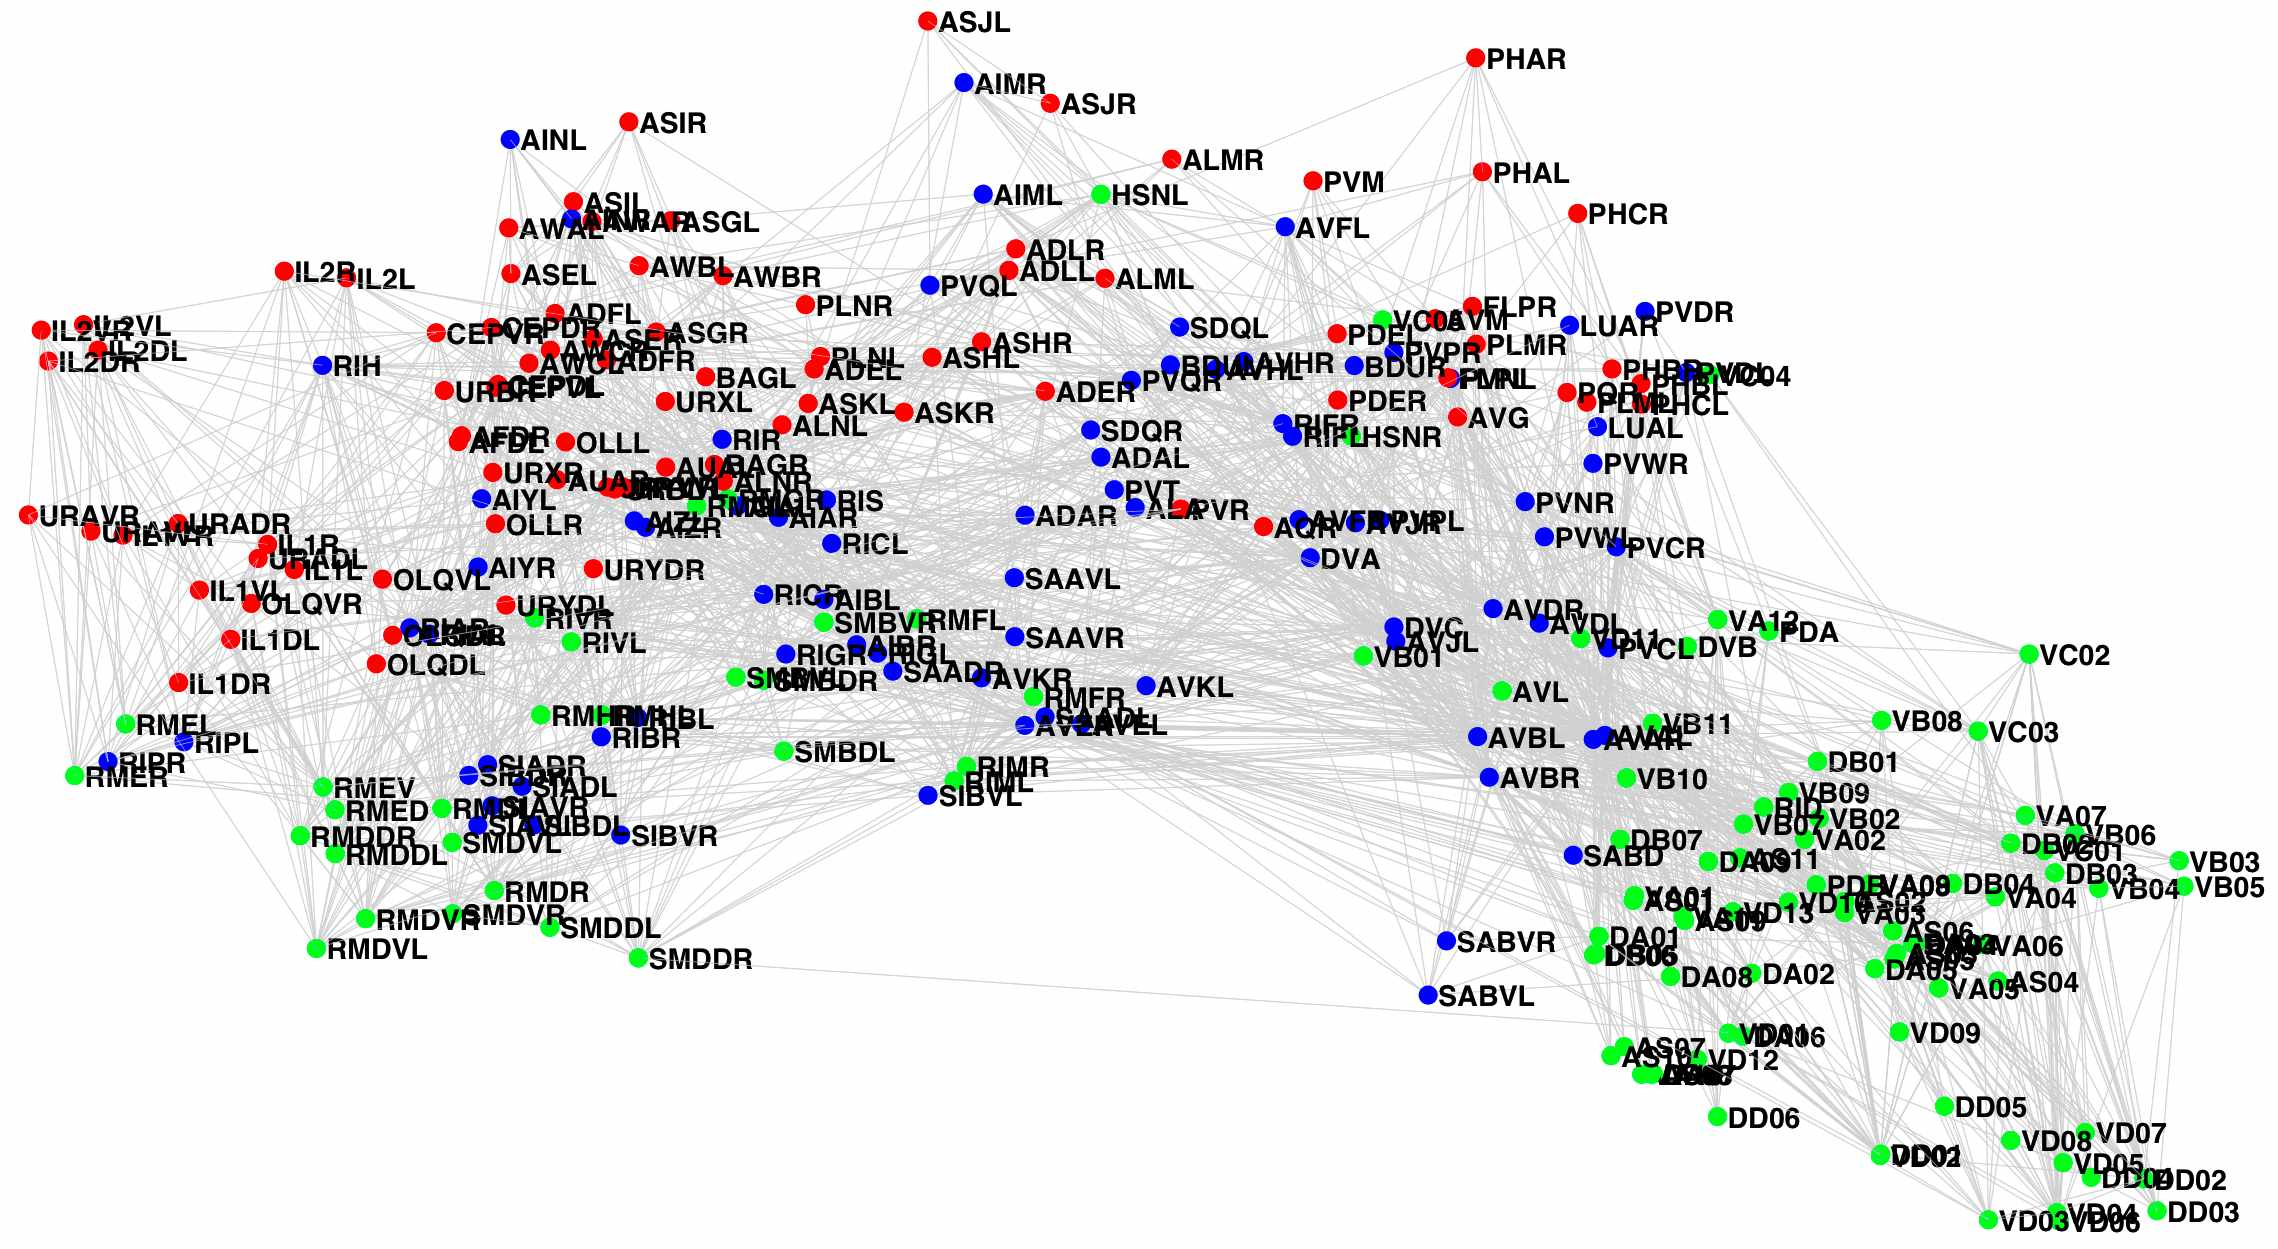
\includegraphics[scale=0.12]{{./figures/celegans}.png}
\end{center}
\end{frame}

\begin{frame}[fragile]
Example: coauthorship graph

\smallskip

\begin{center}
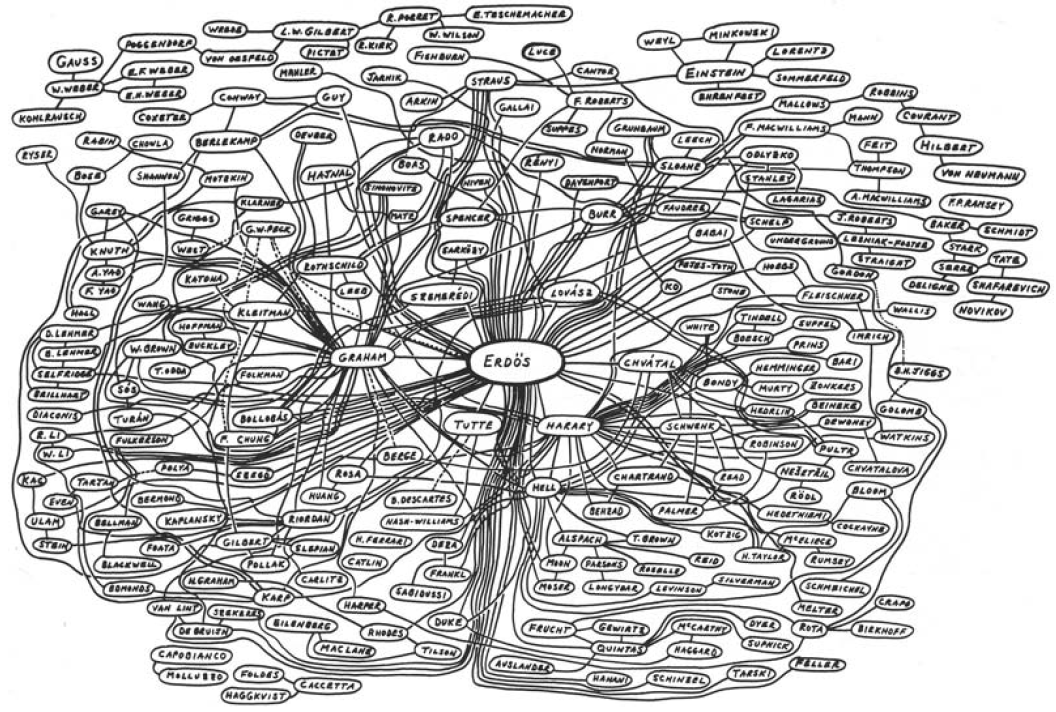
\includegraphics[scale=0.25]{{./figures/erdos}.png}
\end{center}
\end{frame}

\begin{frame}[fragile]
Some graph-processing problems
\begin{center}
\begin{tabular}{cc}
problem & description \\ \hline \\
$s$-$t$ path & is there a path between $s$ and $t$? \\ 
shortest $s$-$t$ path & what is the shortest path between $s$ and $t$? \\
cycle & is there a cycle in the graph? \\
Euler cycle & is there a cycle that uses each edge exactly once? \\
Hamilton cycle & is there a cycle that uses each vertex exactly once? \\
connectivity & is there a way to connect all of the vertices? \\
biconnectivity & is there a vertex whose removal disconnects the graph? \\
bipartiteness & is a graph bipartite? \\ 
planarity & can the graph be drawn in the plane with no crossing edges? \\
graph isomorphism & do two graph representations denote the same graph?
\end{tabular}  
\end{center}
\end{frame}

\section{Undirected Graphs}
\begin{frame}[fragile]
Undirected graph API
\begin{center}
\begin{tabular}{cc}
method & description \\ \hline
\lstinline$Graph(int V)$ & creates a $V$-vertex graph with no edges \\ 
\lstinline$Graph(In in)$ & reads a graph from input stream $in$ \\
\lstinline$int V()$      & returns number of vertices \\
\lstinline$int E()$      & returns number of edges \\
\lstinline$void addEdge(int v, int w)$ & adds edge $v$-$w$ to this graph \\
\lstinline$Iterable<Integer> adj(int v)$ & returns vertices adjacent to $v$
\end{tabular} 
\end{center}

Graph input format
\begin{minipage}{150pt}
\begin{lstlisting}[language={}]
$ more tinyG.txt
13 13 
0 5 4 3 0 1 9 12 6 4 5 4 0 2 
11 12 9 10 0 6 7 8 9 11 5 3
\end{lstlisting}
\end{minipage}%
\begin{minipage}{150pt}
\begin{center}
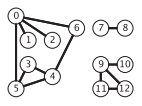
\includegraphics[scale=0.5]{{./figures/graph4}.png}
\end{center}
\end{minipage}

\bigskip

Typical graph-processing code
\begin{lstlisting}[language=Java]
public static int degree(Graph G, int v) {
    int degree = 0;
    for (int w : G.adj(v)) { degree++; }
    return degree;
}
\end{lstlisting}
\end{frame}

\begin{frame}[fragile]
Graph representations
\begin{itemize}
\item Edge list: maintain a list of the edges (linked list or array)

\item Adjacency matrix: maintain a $V$-by-$V$ matrix $M$, such that $M[v][w]$ is 1 if there is an edge from $v$ to $w$, and 0 otherwise

\item Adjacency list: maintain a vertex-indexed array of lists
\end{itemize}

\begin{center}
\begin{tabular}{ccccc}
representation & space & add edge & is $v$-$w$ an edge? & enumerate \lstinline$adj(v)$ \\ \hline \\
edge list & $E$ & 1 & $E$ & $E$ \\
adjacency matrix & $V^2$ & 1$^\dagger$ & 1 & $V$ \\ 
adjacency list & $E+V$ & 1 & $degree(v)$ & $degree(v)$ 
\end{tabular}  

\smallskip

\small $\dagger$ disallows parallel edges
\end{center}
\end{frame}

\begin{frame}[fragile]
\begin{lstlisting}[language=Java]
package edu.princeton.cs.algs4;

public class Graph {
    private final int V;
    private int E;
    private LinkedBag<Integer>[] adj;

    public Graph(int V) {
        if (V < 0) {
            throw new IllegalArgumentException(...); 
        }
        this.V = V;
        this.E = 0;
        adj = (LinkedBag<Integer>[]) new LinkedBag[V];
        for (int v = 0; v < V; v++) {
            adj[v] = new LinkedBag<Integer>();
        }
    }

    public Graph(In in) {
        this(in.readInt());
        int E = in.readInt();
        if (E < 0) { 
            throw new IllegalArgumentException(...);
        }
        for (int i = 0; i < E; i++) {
            int v = in.readInt();
            int w = in.readInt();
            addEdge(v, w);
        }
    }
\end{lstlisting}
\end{frame}

\begin{frame}[fragile]
\begin{lstlisting}[language=Java]
    public int V() { return V; }

    public int E() { return E; }
 
    private void validateVertex(int v) {
        if (v < 0 || v >= V) {
            throw new IndexOutOfBoundsException(...);
        }
    }

    public void addEdge(int v, int w) {
        validateVertex(v);
        validateVertex(w);
        E++;
        adj[v].add(w);
        adj[w].add(v);
    }

    public Iterable<Integer> adj(int v) {
        validateVertex(v);
        return adj[v];
    }
    ...
}
\end{lstlisting}
\end{frame}

\section{Depth-First Search (DFS)}
\begin{frame}[fragile]
\begin{minipage}{210pt}
Goal: systematically traverse a graph

\bigskip

Idea: mimic maze exploration

\bigskip

Typical applications
\begin{itemize}
\item Find all vertices connected to a given source vertex
\item Find a path between two vertices
\end{itemize}

\bigskip

To visit a vertex $v$
\begin{itemize}
\item Mark vertex $v$ as visited
\item Recursively visit all unmarked vertices adjacent to $v$
\end{itemize}

\bigskip

Data structures
\begin{itemize}
\item Boolean array \lstinline{marked[][]} to mark visited vertices
\item Integer array \lstinline{edgeTo[]} to keep track of paths; \lstinline{edgeTo[w] = v} means that edge $v$-$w$ taken to visit $w$ for first time
\item Function-call stack for recursion
\end{itemize}
\end{minipage}
\begin{minipage}{90pt}
\begin{center}
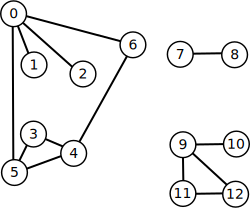
\includegraphics[scale=0.4]{{./figures/graph5}.png}

\smallskip

\small depth-first maze exploration
\end{center}
\end{minipage}
\end{frame}

\begin{frame}[fragile]
Design pattern for graph processing: decouple graph data type from graph processing
\begin{itemize}
\item Create a \lstinline{Graph} object
\item Pass the \lstinline{Graph} object to a graph-processing routine
\item Query the graph-processing routine for information
\end{itemize}

\begin{center}
\begin{tabular}{cc}
method & description \\ \hline
\lstinline$Paths(Graph G, int s)$ & finds paths in $G$ from source $s$ \\
\lstinline$boolean hasPathTo(int v)$ & is there a path from $s$ to $v$? \\
\lstinline$Iterable<Integer> pathTo(int v)$ & returns path from $s$ to $v$, or \lstinline$null$
\end{tabular} 
\end{center}

\bigskip

Typical graph-processing code
\begin{lstlisting}[language=Java]
    ...
    Paths paths = new Paths(G, s);
    for (int v = 0; v < G.V(); v++) {
        if (paths.hasPathTo(v)) {
            StdOut.println(v);
        }
    }
    ...
\end{lstlisting}
\end{frame}

\begin{frame}[fragile]
\begin{lstlisting}[language=Java]
package edu.princeton.cs.algs4;

public class DepthFirstPaths {
    private boolean[] marked; 
    private int[] edgeTo; 
    private final int s; 

    public DepthFirstPaths(Graph G, int s) {
        this.s = s;
        edgeTo = new int[G.V()];
        marked = new boolean[G.V()];
        dfs(G, s);
    }

    private void dfs(Graph G, int v) {
        marked[v] = true;
        for (int w : G.adj(v)) {
            if (!marked[w]) {
                edgeTo[w] = v;
                dfs(G, w);
            }
        }
    }

    public boolean hasPathTo(int v) { return marked[v]; }

    public Iterable<Integer> pathTo(int v) {
        if (!hasPathTo(v)) { return null; }
        LinkedStack<Integer> path = new LinkedStack<Integer>();
        for (int x = v; x != s; x = edgeTo[x]) { path.push(x); }
        path.push(s);
        return path;
    }
    ...
}
\end{lstlisting}
\end{frame}

\begin{frame}[fragile]
\begin{center}
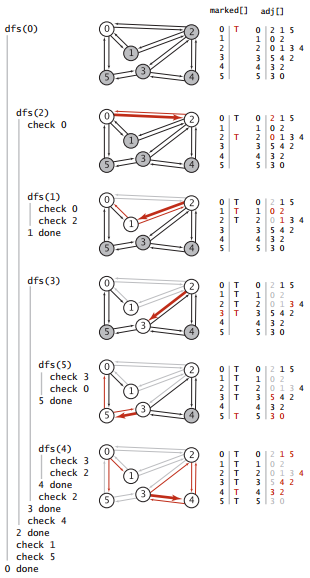
\includegraphics[scale=0.37]{{./figures/graph6}.png}

\smallskip

\small trace of depth-first search to find vertices connected to 0
\end{center}
\end{frame}

\section{Breadth-First Search (BFS)}
\begin{frame}[fragile]
\begin{minipage}{210pt}
Goal: given a graph and a source vertex $s$, support queries of the form
\begin{itemize}
\item Is there a path from $s$ to a given target vertex $v$?

\item If so, find a shortest such path (one with minimal number of edges)
\end{itemize}

\bigskip

Repeat until queue is empty
\begin{itemize}
\item Remove vertex $v$ from queue

\item Add to queue all unmarked vertices adjacent to v and mark them
\end{itemize}
\end{minipage}
\begin{minipage}{90pt}
\begin{center}
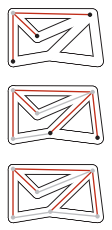
\includegraphics[scale=0.4]{{./figures/graph7}.png}

\smallskip

\small breadth-first maze exploration
\end{center}
\end{minipage}
\end{frame}

\begin{frame}[fragile]
\begin{lstlisting}[language=Java]
package edu.princeton.cs.algs4;

public class BreadthFirstPaths {
    private static final int INFINITY = Integer.MAX_VALUE;
    private boolean[] marked; 
    private int[] edgeTo; 
    private int[] distTo;   

    public BreadthFirstPaths(Graph G, int s) {
        marked = new boolean[G.V()];
        distTo = new int[G.V()];
        edgeTo = new int[G.V()];
        bfs(G, s);
    }

    private void bfs(Graph G, int s) {
        LinkedQueue<Integer> q = new LinkedQueue<Integer>();
        for (int v = 0; v < G.V(); v++) { distTo[v] = INFINITY; }
        distTo[s] = 0;
        marked[s] = true;
        q.enqueue(s);
        while (!q.isEmpty()) {
            int v = q.dequeue();
            for (int w : G.adj(v)) {
                if (!marked[w]) {
                    edgeTo[w] = v;
                    distTo[w] = distTo[v] + 1;
                    marked[w] = true;
                    q.enqueue(w);
                }
            }
        }
    }
\end{lstlisting}
\end{frame}

\begin{frame}[fragile]
\begin{lstlisting}[language=Java]
    public boolean hasPathTo(int v) { return marked[v]; }

    public int distTo(int v) { return distTo[v]; }

    public Iterable<Integer> pathTo(int v) {
        if (!hasPathTo(v)) return null;
        LinkedStack<Integer> path = new LinkedStack<Integer>();
        int x;
        for (x = v; distTo[x] != 0; x = edgeTo[x]) {
            path.push(x);
        }
        path.push(x);
        return path;
    }
    ...
}
\end{lstlisting}
\end{frame}

\begin{frame}[fragile]
\begin{center}
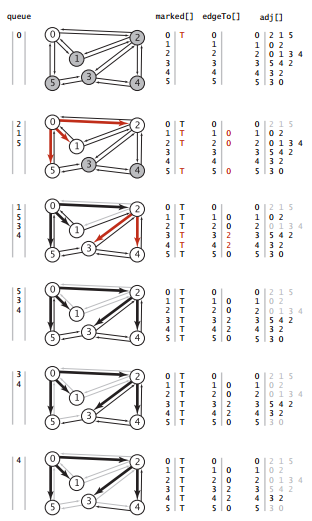
\includegraphics[scale=0.37]{{./figures/graph8}.png}

\smallskip

\small trace of breadth-first search to find all paths from 0
\end{center}
\end{frame}

\section{Connected Components}
\begin{frame}[fragile]
Vertices $v$ and $w$ are \emph{connected} if there is a path between them

\bigskip

Goal: preprocess graph to answer queries of the form \emph{is $v$ connected to $w$} in constant time

\begin{center}
\begin{tabular}{cc}
method & description \\ \hline
\lstinline$CC(Graph G)$ & finds connected components in $G$ \\
\lstinline$boolean connected(int v, int w)$ & are $v$ and $w$ connected? \\
\lstinline$int count()$ & returns the number of connected components \\
\lstinline$int id(int v)$ & returns the component identifier for $v$ \\
\lstinline$int size(int v)$ & returns the number of vertices in $v$'s component
\end{tabular} 
\end{center}

\bigskip

Use union-find? not quite

\bigskip

Use depth-first search? yes
\end{frame}

\begin{frame}[fragile]
\begin{lstlisting}[language=Java]
package edu.princeton.cs.algs4;

public class CC {
    private boolean[] marked; 
    private int[] id; 
    private int[] size;  
    private int count;  
    
   public CC(Graph G) {
        marked = new boolean[G.V()];
        id = new int[G.V()];
        size = new int[G.V()];
        for (int v = 0; v < G.V(); v++) {
            if (!marked[v]) {
                dfs(G, v);
                count++;
            }
        }
    }

    private void dfs(Graph G, int v) {
        marked[v] = true;
        id[v] = count;
        size[count]++;
        for (int w : G.adj(v)) { if (!marked[w]) { dfs(G, w); } }
    }
    
    public boolean connected(int v, int w) { return id(v) == id(w); }

    public int count() { return count; }

    public int id(int v) { return id[v]; }

    public int size(int v) { return size[id[v]]; }
    ...
}
\end{lstlisting} 
\end{frame}

\section{Graph Traversal Summary}
\begin{frame}[fragile]
BFS and DFS enables efficient solution of many (but not all) graph problems
\begin{center}
\begin{tabular}{cccc}
problem & BFS & DFS & time \\ \hline \\
path between $s$ and $t$ & \cmark & \cmark & $E + V$ \\
shortest path between $s$ and $t$ & \cmark & & $E+V$ \\
cycle & \cmark & \cmark & $E+V$ \\
Euler cycle & & \cmark & $E+V$ \\
Hamilton cycle & & & $2^{1.657V}$ \\
connected components & \cmark & \cmark & $E+V$ \\
biconnected components & & \cmark & $E+V$ \\
bipartiteness & \cmark & \cmark & $E+V$ \\
planarity & & \cmark & $E+V$ \\
graph isomorphism & & & $2^{c\sqrt{V\log V}}$ 
\end{tabular} 
\end{center}
\end{frame}

\end{document}
